\chapter{Wing Box model}
\label{chap:model}

\section{Introduction} \label{sec:introInModel}

% Introduction to the chapter

\section{Concept} \label{sec:conceptInModel}

% Explanation of the concept
% -> Bending-twist coupling
% -> Shiftable shear centre location
% -> A web with variable-stiffness capability

% Figure: Fig. 1 Raither ?, Geometry and system of coordinates.
% Figure: Fig. 2 Raither ?, Schematic of the working principle.

% -> Buckling phenomena
% Figure: Schematic representation buckling phenomena

\section{Analytical model} \label{sec:analyticalModel}

%% Analytical apprach description
% An analytical model of the Wing Box will be build.
% The twist of the beam will be calculated
%
%Figure of analytical model
\begin{figure}[!htpb]
  \centering
  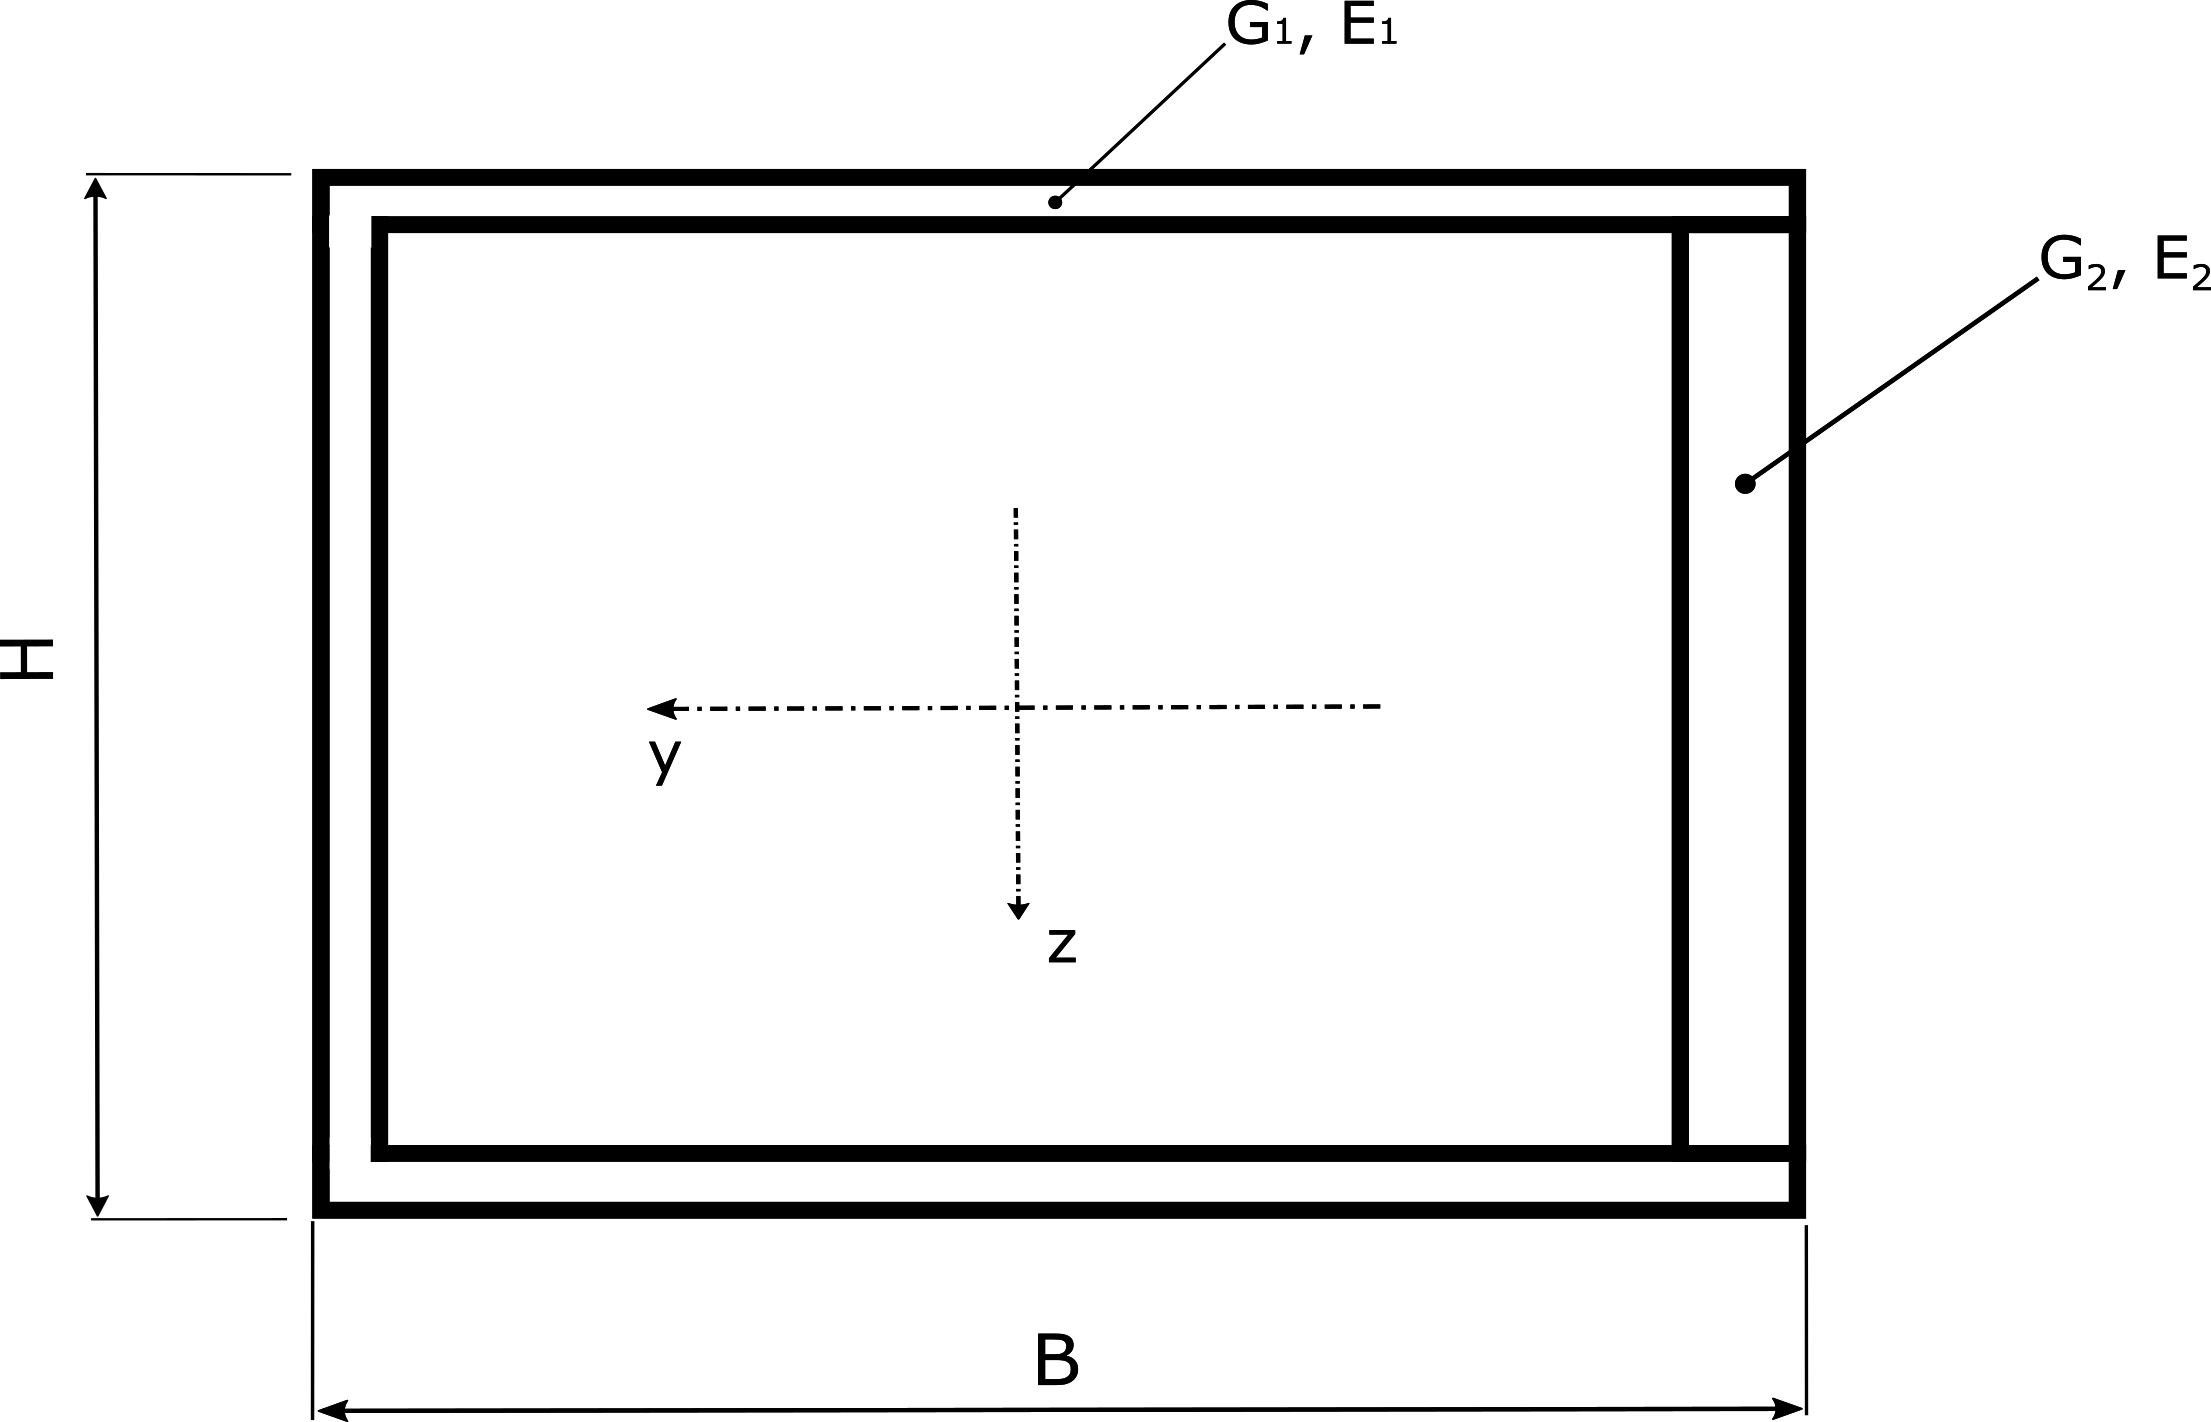
\includegraphics[width=0.8 \textwidth]{model/analyticalBox}
  \caption[Schematic view of the beam closed section]{Schematic view of the beam closed section. The dimensions are given by the width $B$ and the height $H$. For the upper, lower and left elements, the shear modulus and the elastic modulus are given by $G_1$ and $E_1$, respectively. For the right element, the same mechanical properties are given by $G_2$ and $E_2$.}\label{fig:analyticalBox}
\end{figure}

%Torsional stiffness

\begin{equation}\label{eq:torStiff}
  G I_t = \frac{4 A_0^2}{\oint \frac{\mathrm{d} s}{G(s) t(s)}}
\end{equation}

%Equations for the static moment and the flexural stiffness along the $y$ axis $\Phi_y$ (3.17, 3.18, 3.19)

%Equations for the shear flow calculation (3.20, 3.21)

%Shear centre expressions (3.22)

%The shear force is moved to the shear centre, causing an additional torsional moment given by Equation \ref{eq:momentDueToQz}. This produces a constant shear flow $q_M$ that is calculated as shown in Equation \ref{eq:constantShearFlow}.

\begin{equation}\label{eq:momentDueToQz}
  M_\mathrm{t} = Q_\mathrm{z} (y_{\mathrm{Q}} - y_\mathrm{SC})
\end{equation}
%
\begin{equation}\label{eq:constantShearFlow}
  q_M = \frac{M_\mathrm{t}}{2 A_0}
\end{equation}
%
where it has been taken into a account that a positive moment along the $x$ axis produces a constant shear flow distribution which has opposite sign as the shear flow distribution defined positive.

Finally, the total shear flow is given by the Expression \ref{eq:totalShearFlow}.

\begin{equation}\label{eq:totalShearFlow}
  q(s) = q_\mathrm{C}(s) - q_\mathrm{M}
\end{equation}

\subsection{Parametric study} \label{subsec:parametricStudy} %Reference for this part -> \cite{Raither_basic}

In the present subsection, the variation of the beam properties for different values parameter values will be shown. The beam geometry will be characterized through the cross-sectional aspect ratio $B/H$ and the thickness ratio $t_2/t_1$. The effect of this parameters on the sectional properties, twist and bending stiffness will be shown. Additionally, the variance of the stiffness ratio $E_1/E_2$ will also be included in the model.

The effect of the slenderness ratio $L/B$ on the torsional and deflection compliances is shown in Figures XX and XX, respectively.

\subsubsection{Results} \label{subsubsec:results_parametricStudy}

The influence of the cross-sectional aspect ratio $B/H$ on the torsional stiffness $G I_t$, the shear centre position $y_{SC}$ and the flexural stiffness $E I_y$ is shown in Figures \ref{fig:GIt-E1overE2-BoverH}, \ref{fig:SC-E1overE2-BoverH} and \ref{fig:EIy-E1overE2-BoverH}, respectively. Furthermore the effect of thickness ratio $t_2/t_1$ on the same three beam parameters is shown in Figures \ref{fig:GIt-E1overE2-t2overt1}, \ref{fig:SC-E1overE2-t2overt1} and \ref{fig:EIy-E1overE2-t2overt1}. 

%Figures variation of B/H
\begin{figure}[!htpb] %G I_t versus B/H
  \centering
  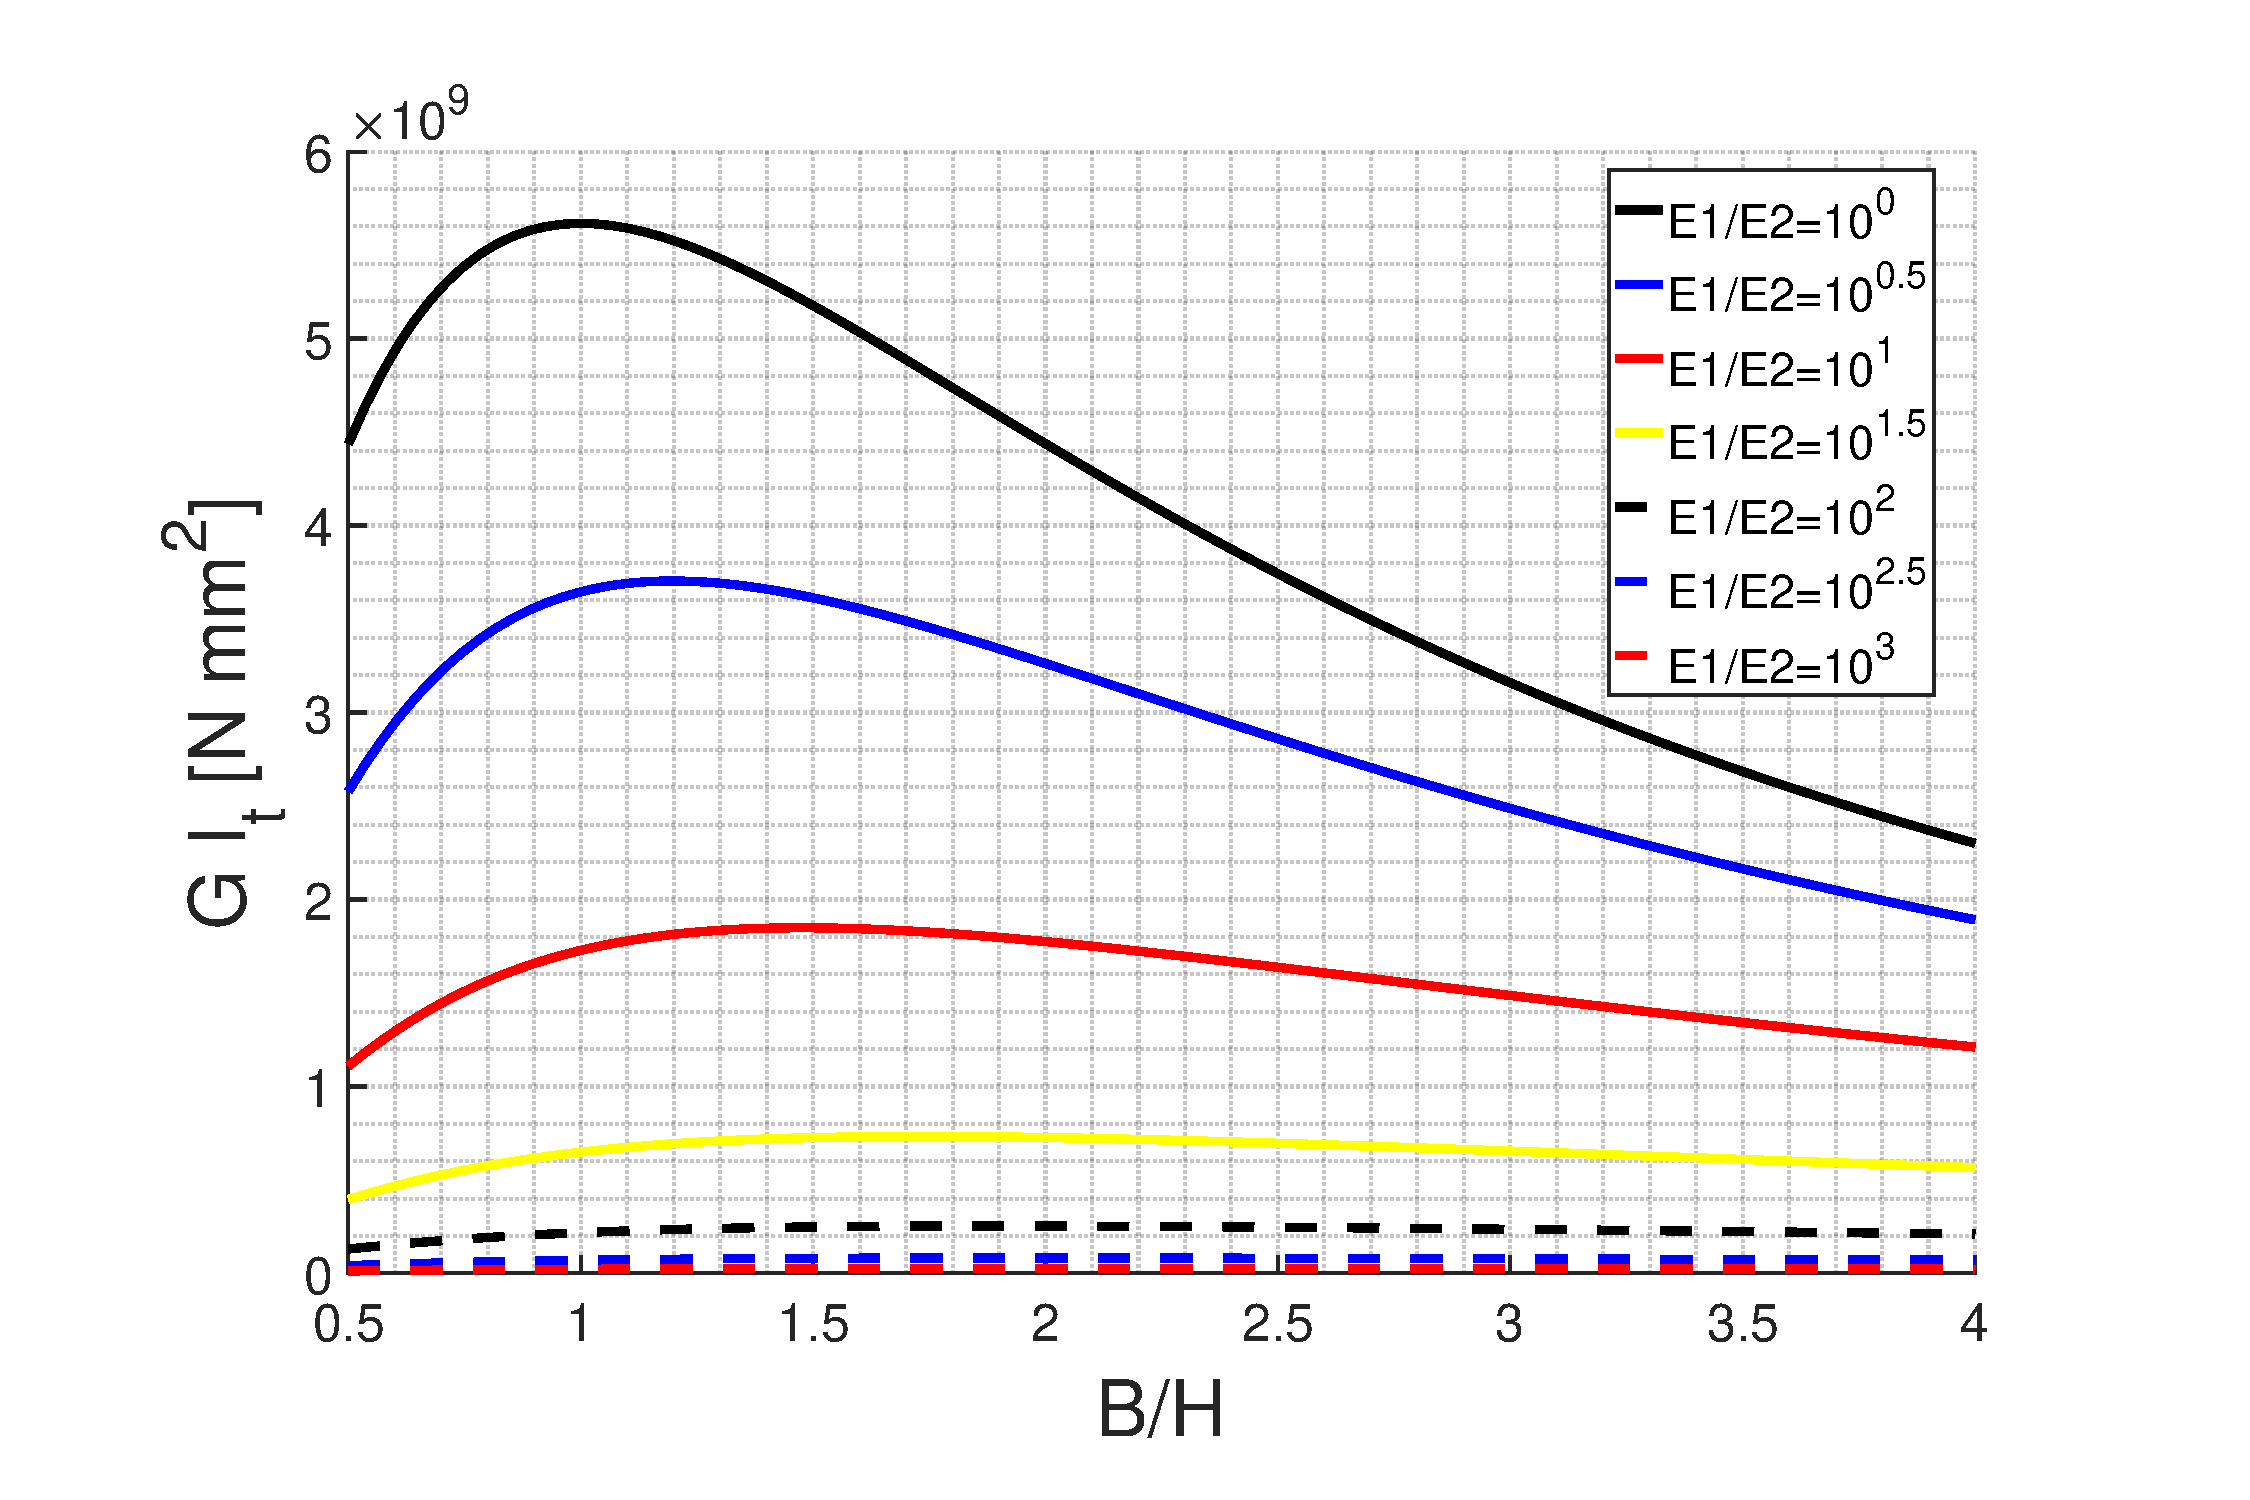
\includegraphics[width=0.8 \textwidth]{../../analytical/figures/GIt-E1overE2-BoverH}
  \caption[Influence of the cross-sectional aspect ratio $B/H$ on the torsional stiffness $GI_t$]{Influence of the cross-sectional aspect ratio $B/H$ on the torsional stiffness $GI_t$ shown for various values of the stiffness ratio $E_1/E_2$ ranging from $10^0$ to $10^3$. }\label{fig:GIt-E1overE2-BoverH}
\end{figure}

\begin{figure}[!htpb] %Shear centre versus B/H
  \centering
  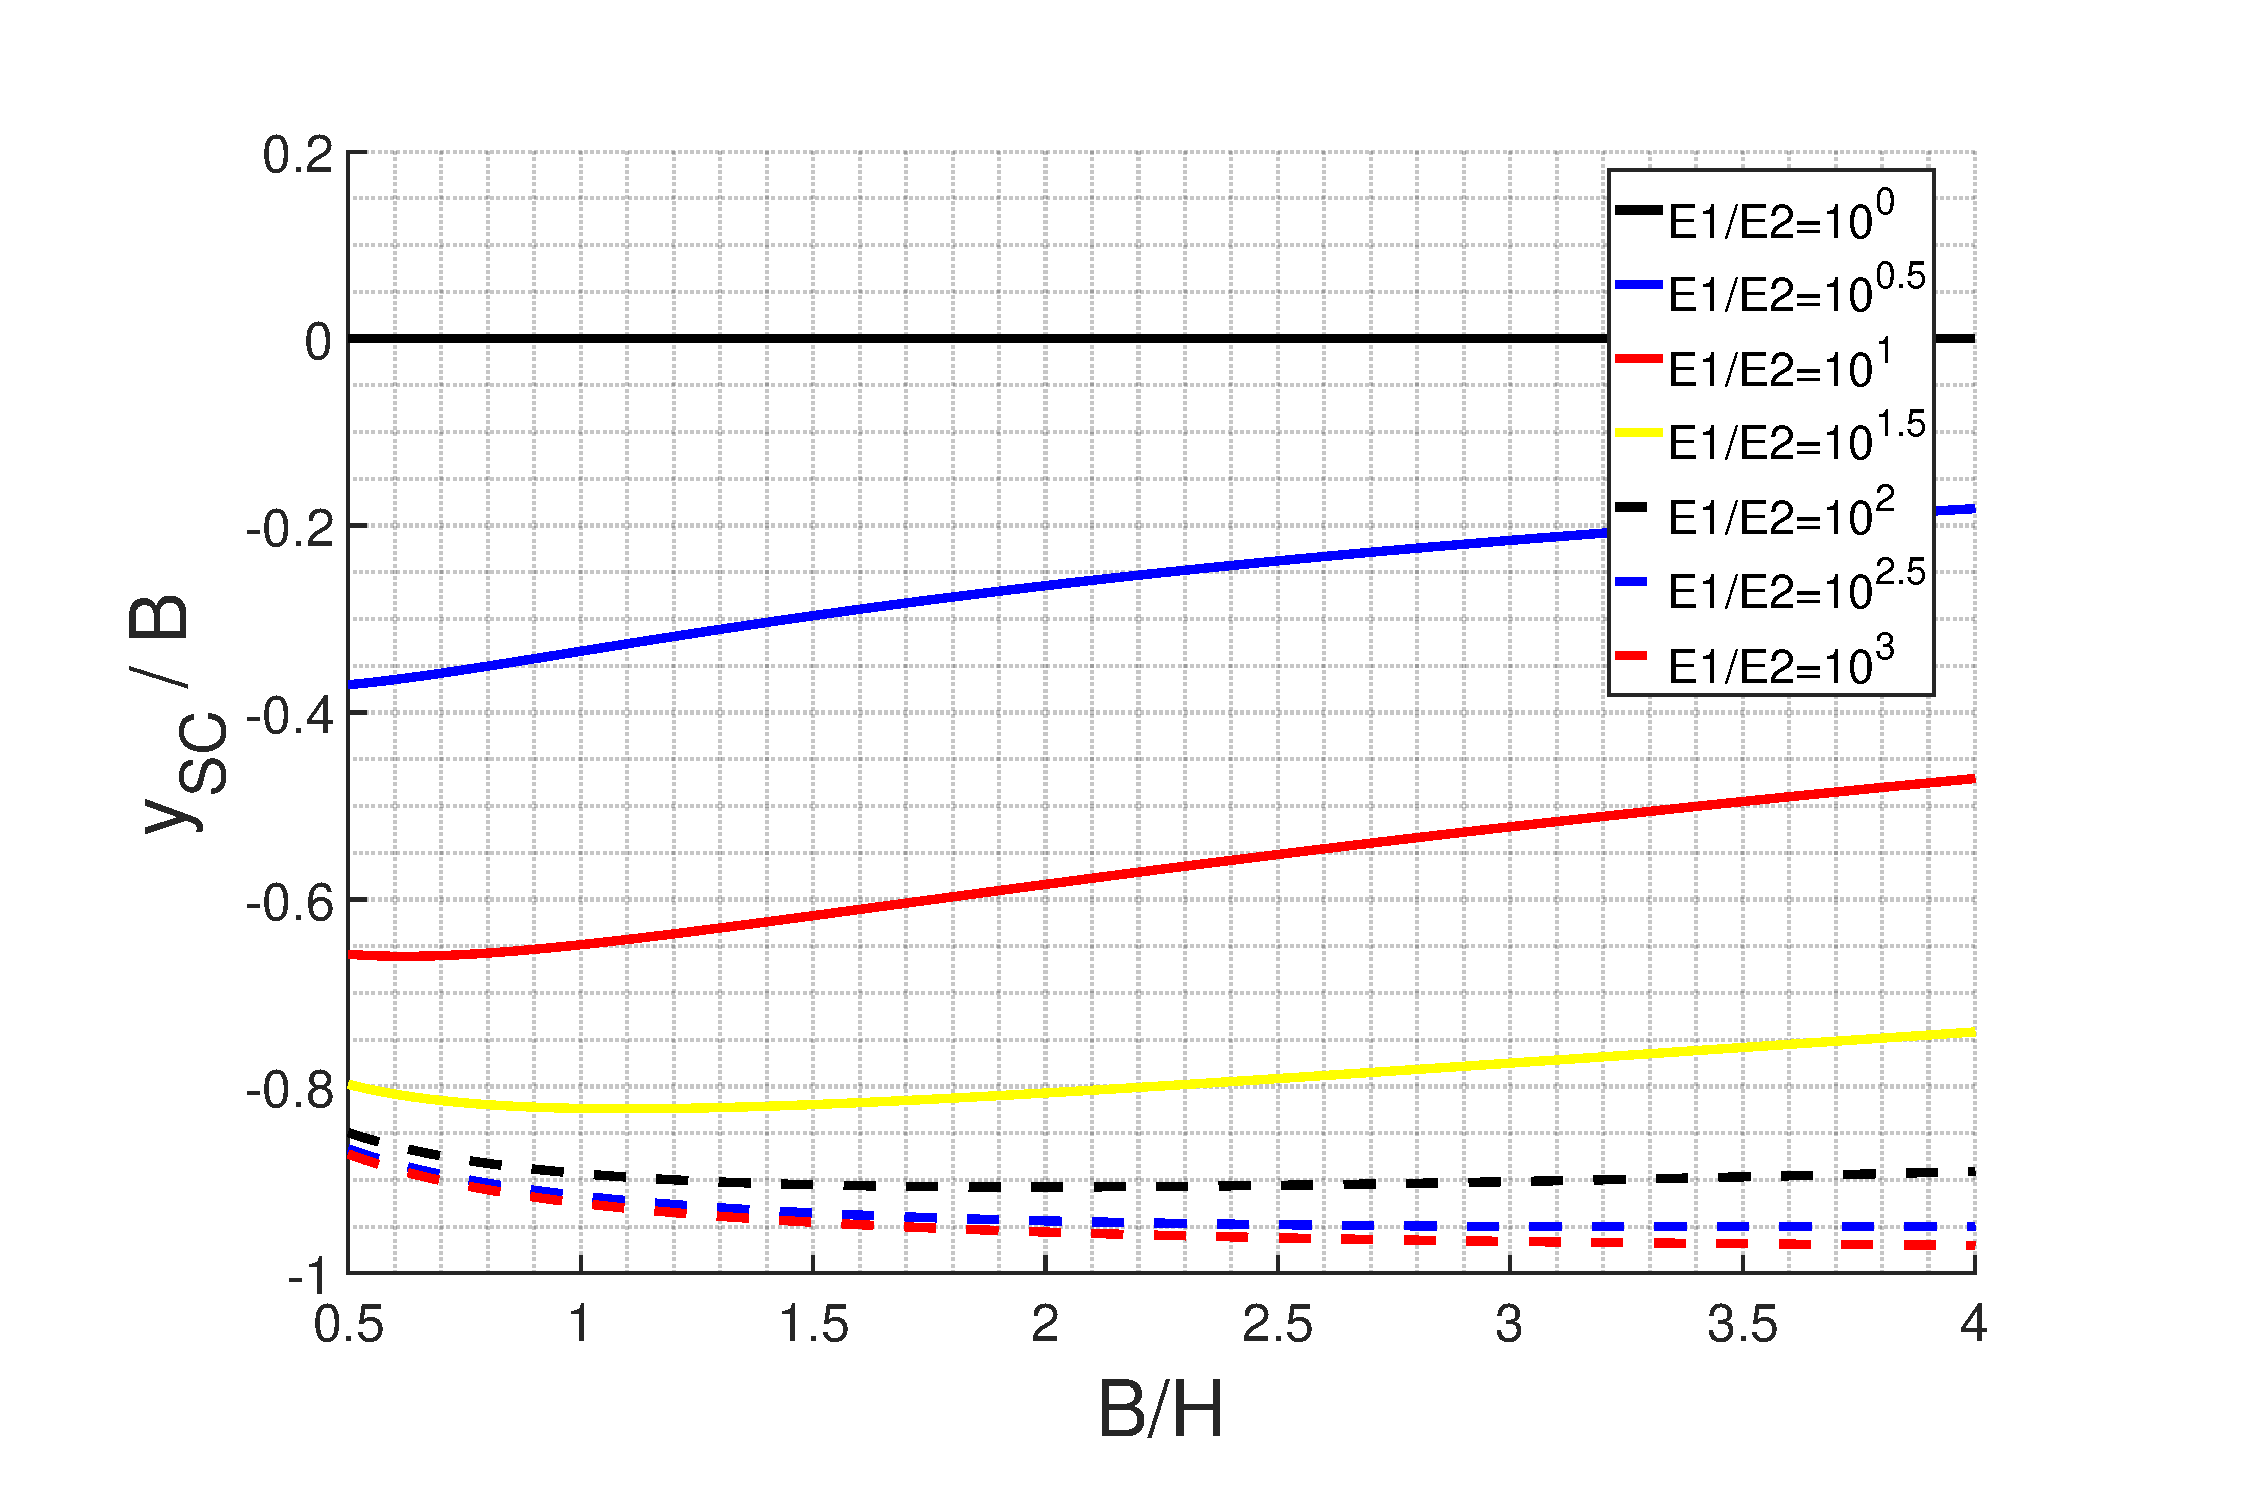
\includegraphics[width=0.8 \textwidth]{../../analytical/figures/SC-E1overE2-BoverH}
  \caption[Influence of the cross-sectional aspect ratio $B/H$ on the dimensionless shear centre position $y_{SC}/B$]{Influence of the cross-sectional aspect ratio $B/H$ on the dimensionless shear centre position $y_{SC}/B$ shown for various values of the stiffness ratio $E_1/E_2$ ranging from $10^0$ to $10^3$. }\label{fig:SC-E1overE2-BoverH}
\end{figure}

\begin{figure}[!htpb] %E I_y = \Phi_y versus B/H
  \centering
  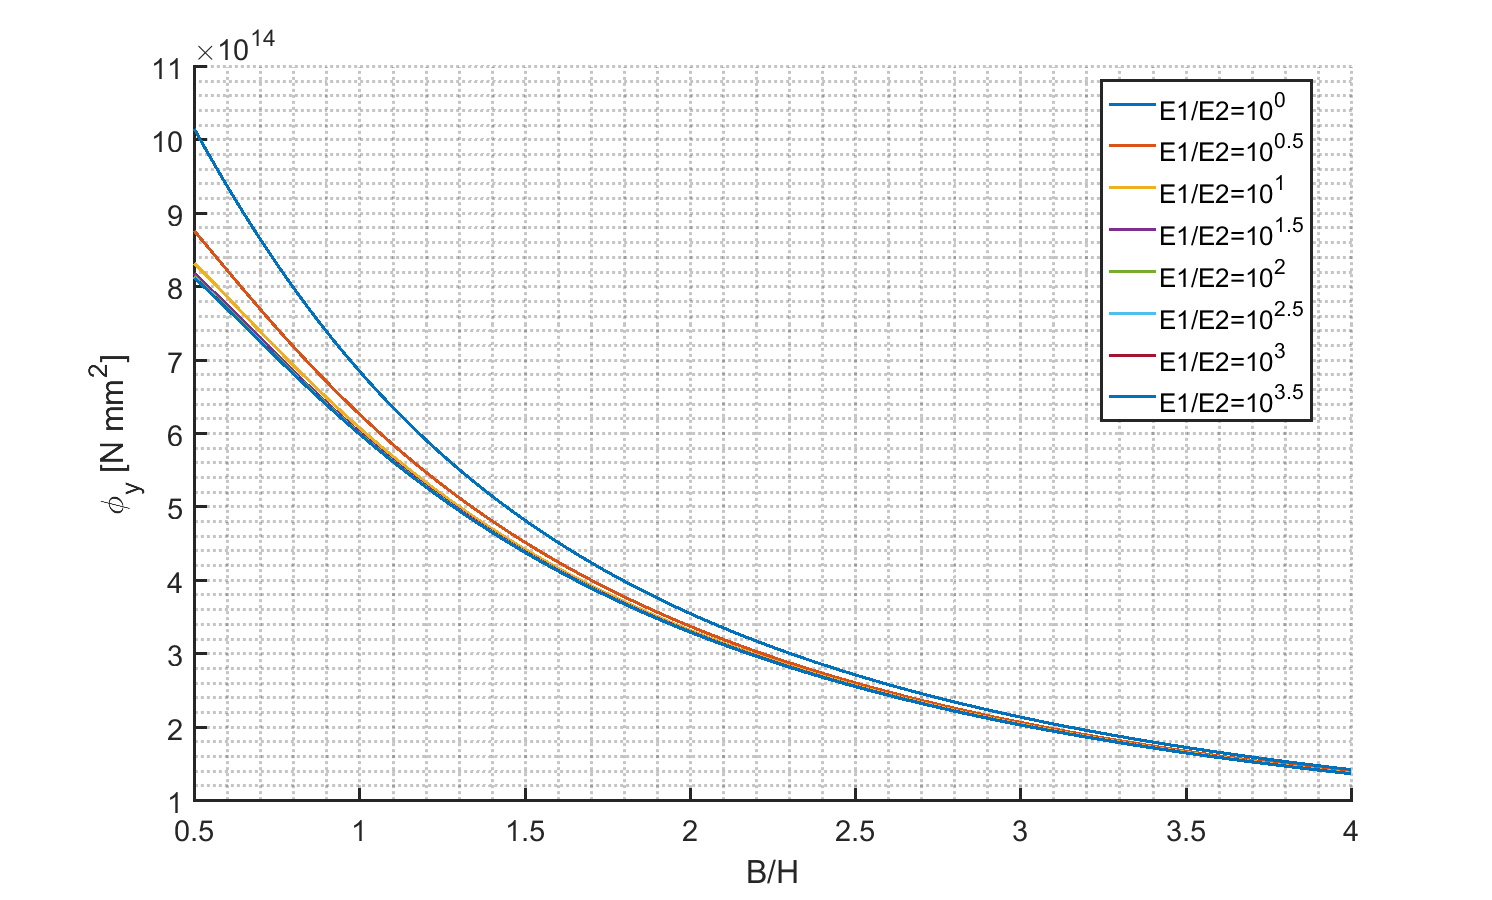
\includegraphics[width=0.8 \textwidth]{../../analytical/figures/EIy-E1overE2-BoverH}
  \caption[Influence of the cross-sectional aspect ratio $B/H$ on the flexural stiffness $EI_y$]{Influence of the cross-sectional aspect ratio $B/H$ on the flexural stiffness $EI_y = \Phi_y$ shown for various values of the stiffness ratio $E_1/E_2$ ranging from $10^0$ to $10^3$. }\label{fig:EIy-E1overE2-BoverH}
\end{figure}

%%%% Figures variation of t2/t1
\begin{figure}[!htpb] %G I_t versus B/H
  \centering
  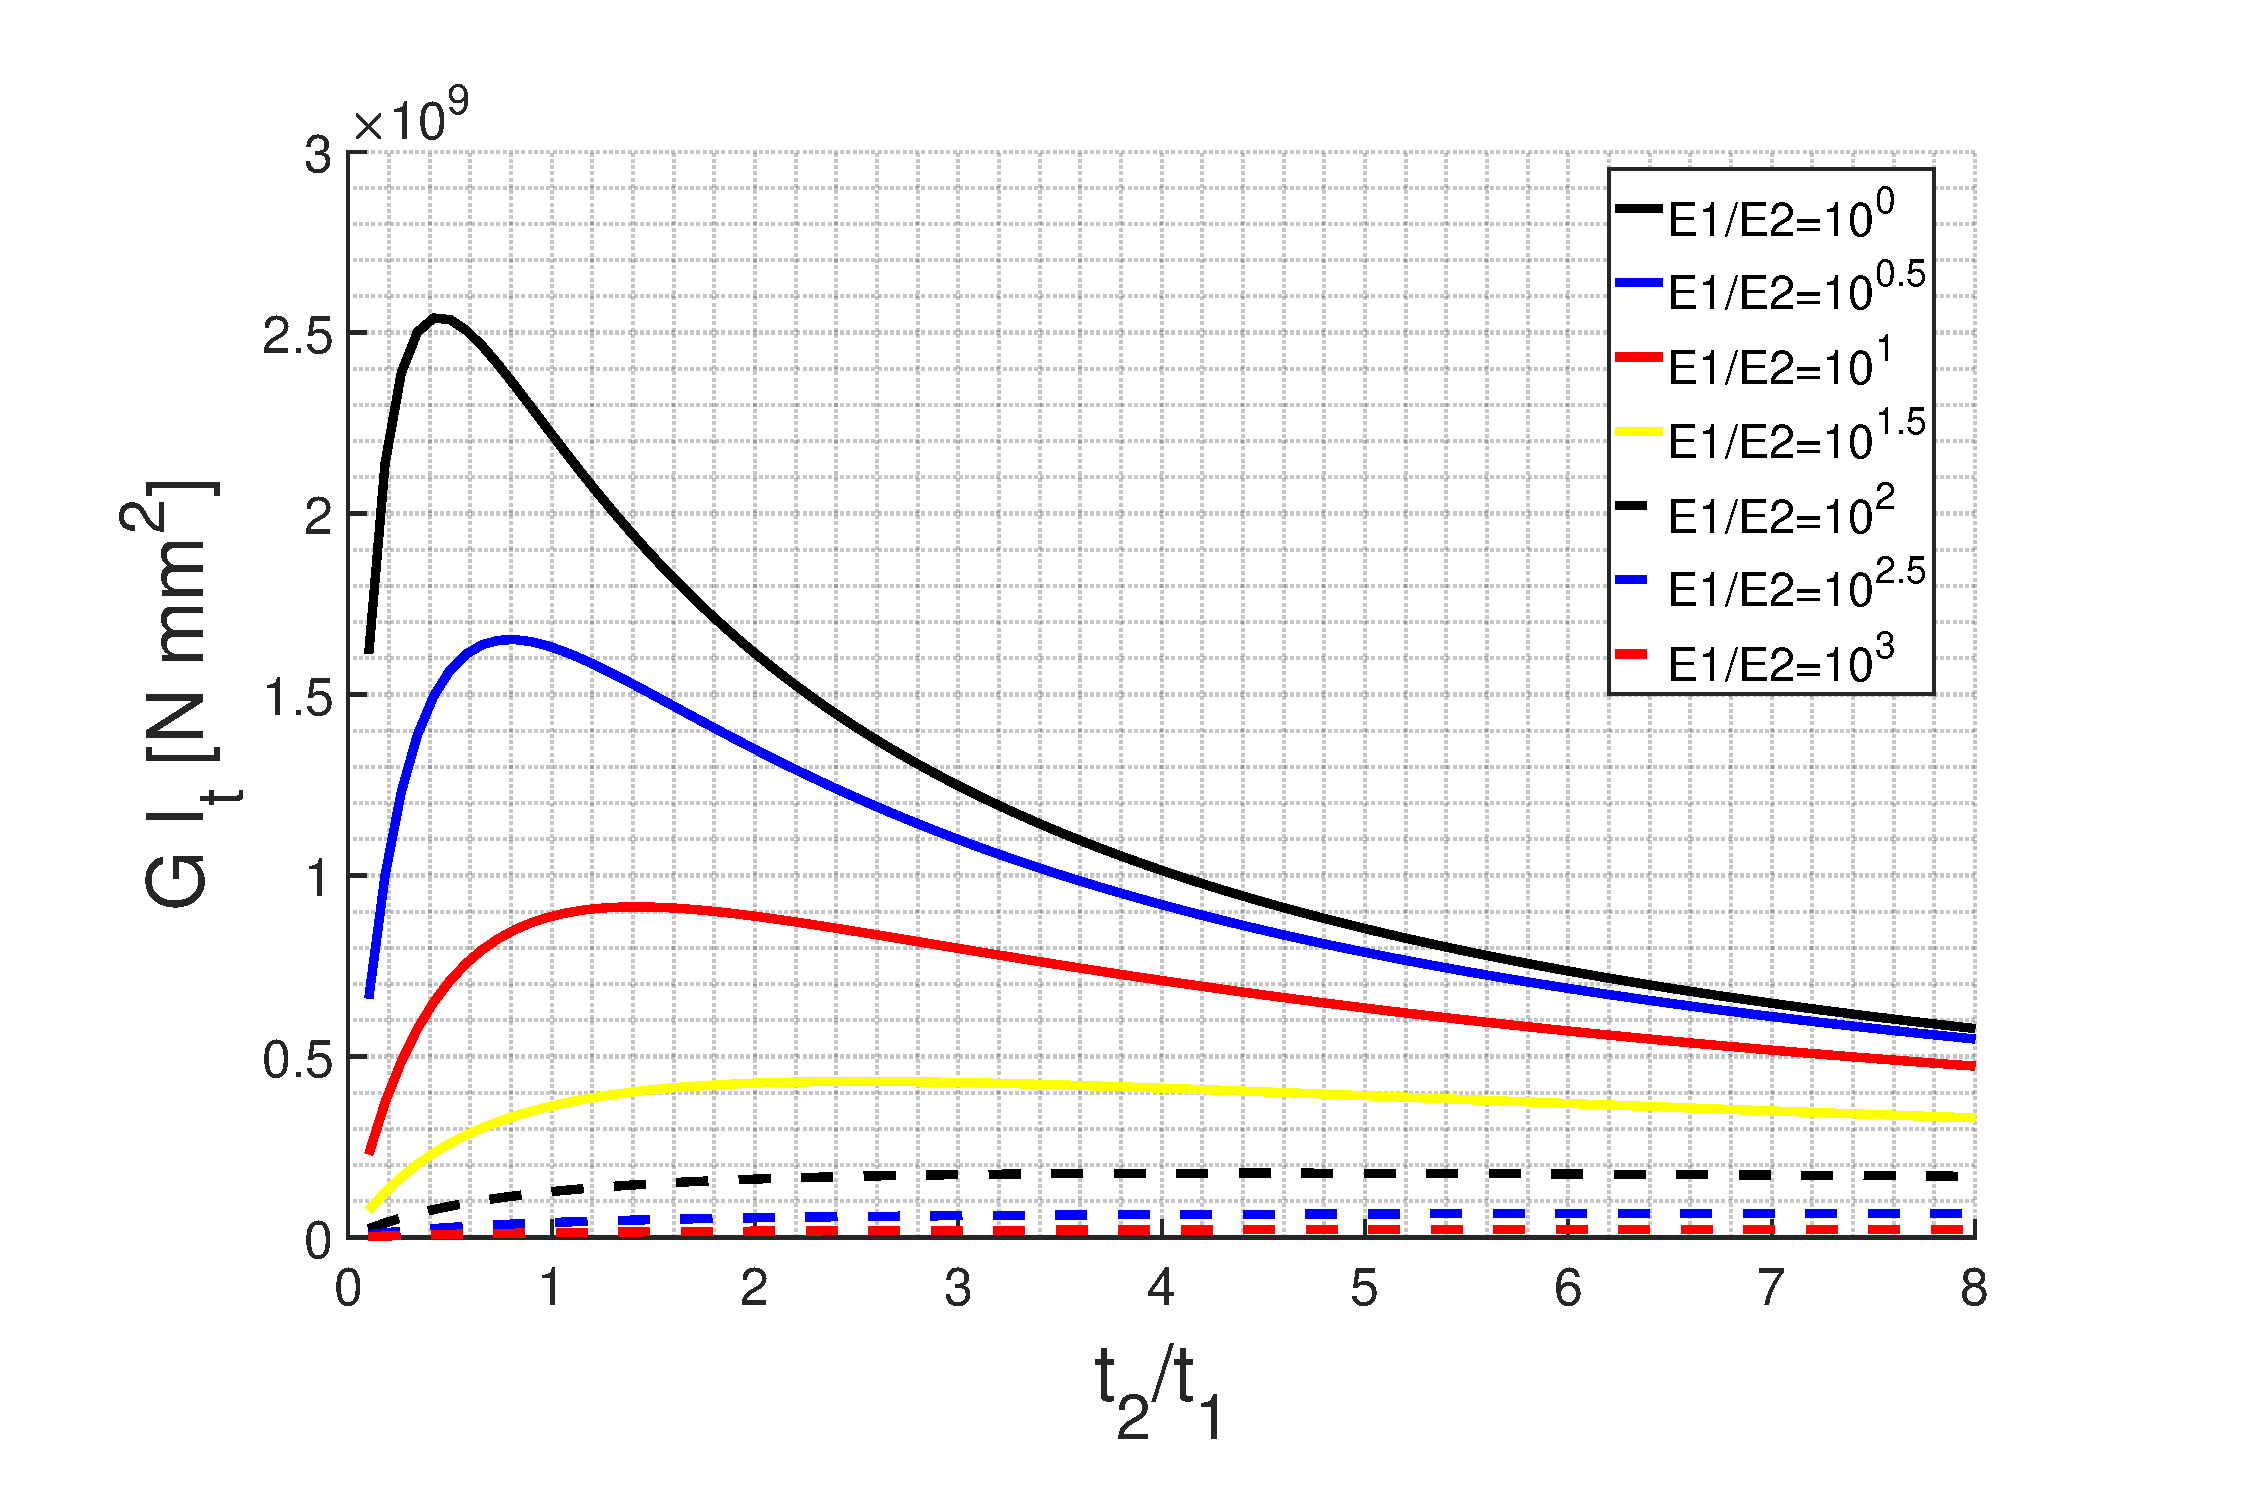
\includegraphics[width=0.8 \textwidth]{../../analytical/figures/GIt-E1overE2-t2overt1}
  \caption[Influence of the wall thickness ratio $t_2/t_1$ on the torsional stiffness $GI_t$]{Influence of the wall thickness ratio $t_2/t_1$ on the torsional stiffness $GI_t$ shown for various values of the stiffness ratio $E_1/E_2$ ranging from $10^0$ to $10^3$. }\label{fig:GIt-E1overE2-t2overt1}
\end{figure}

\begin{figure}[!htpb] %Shear centre versus B/H
  \centering
  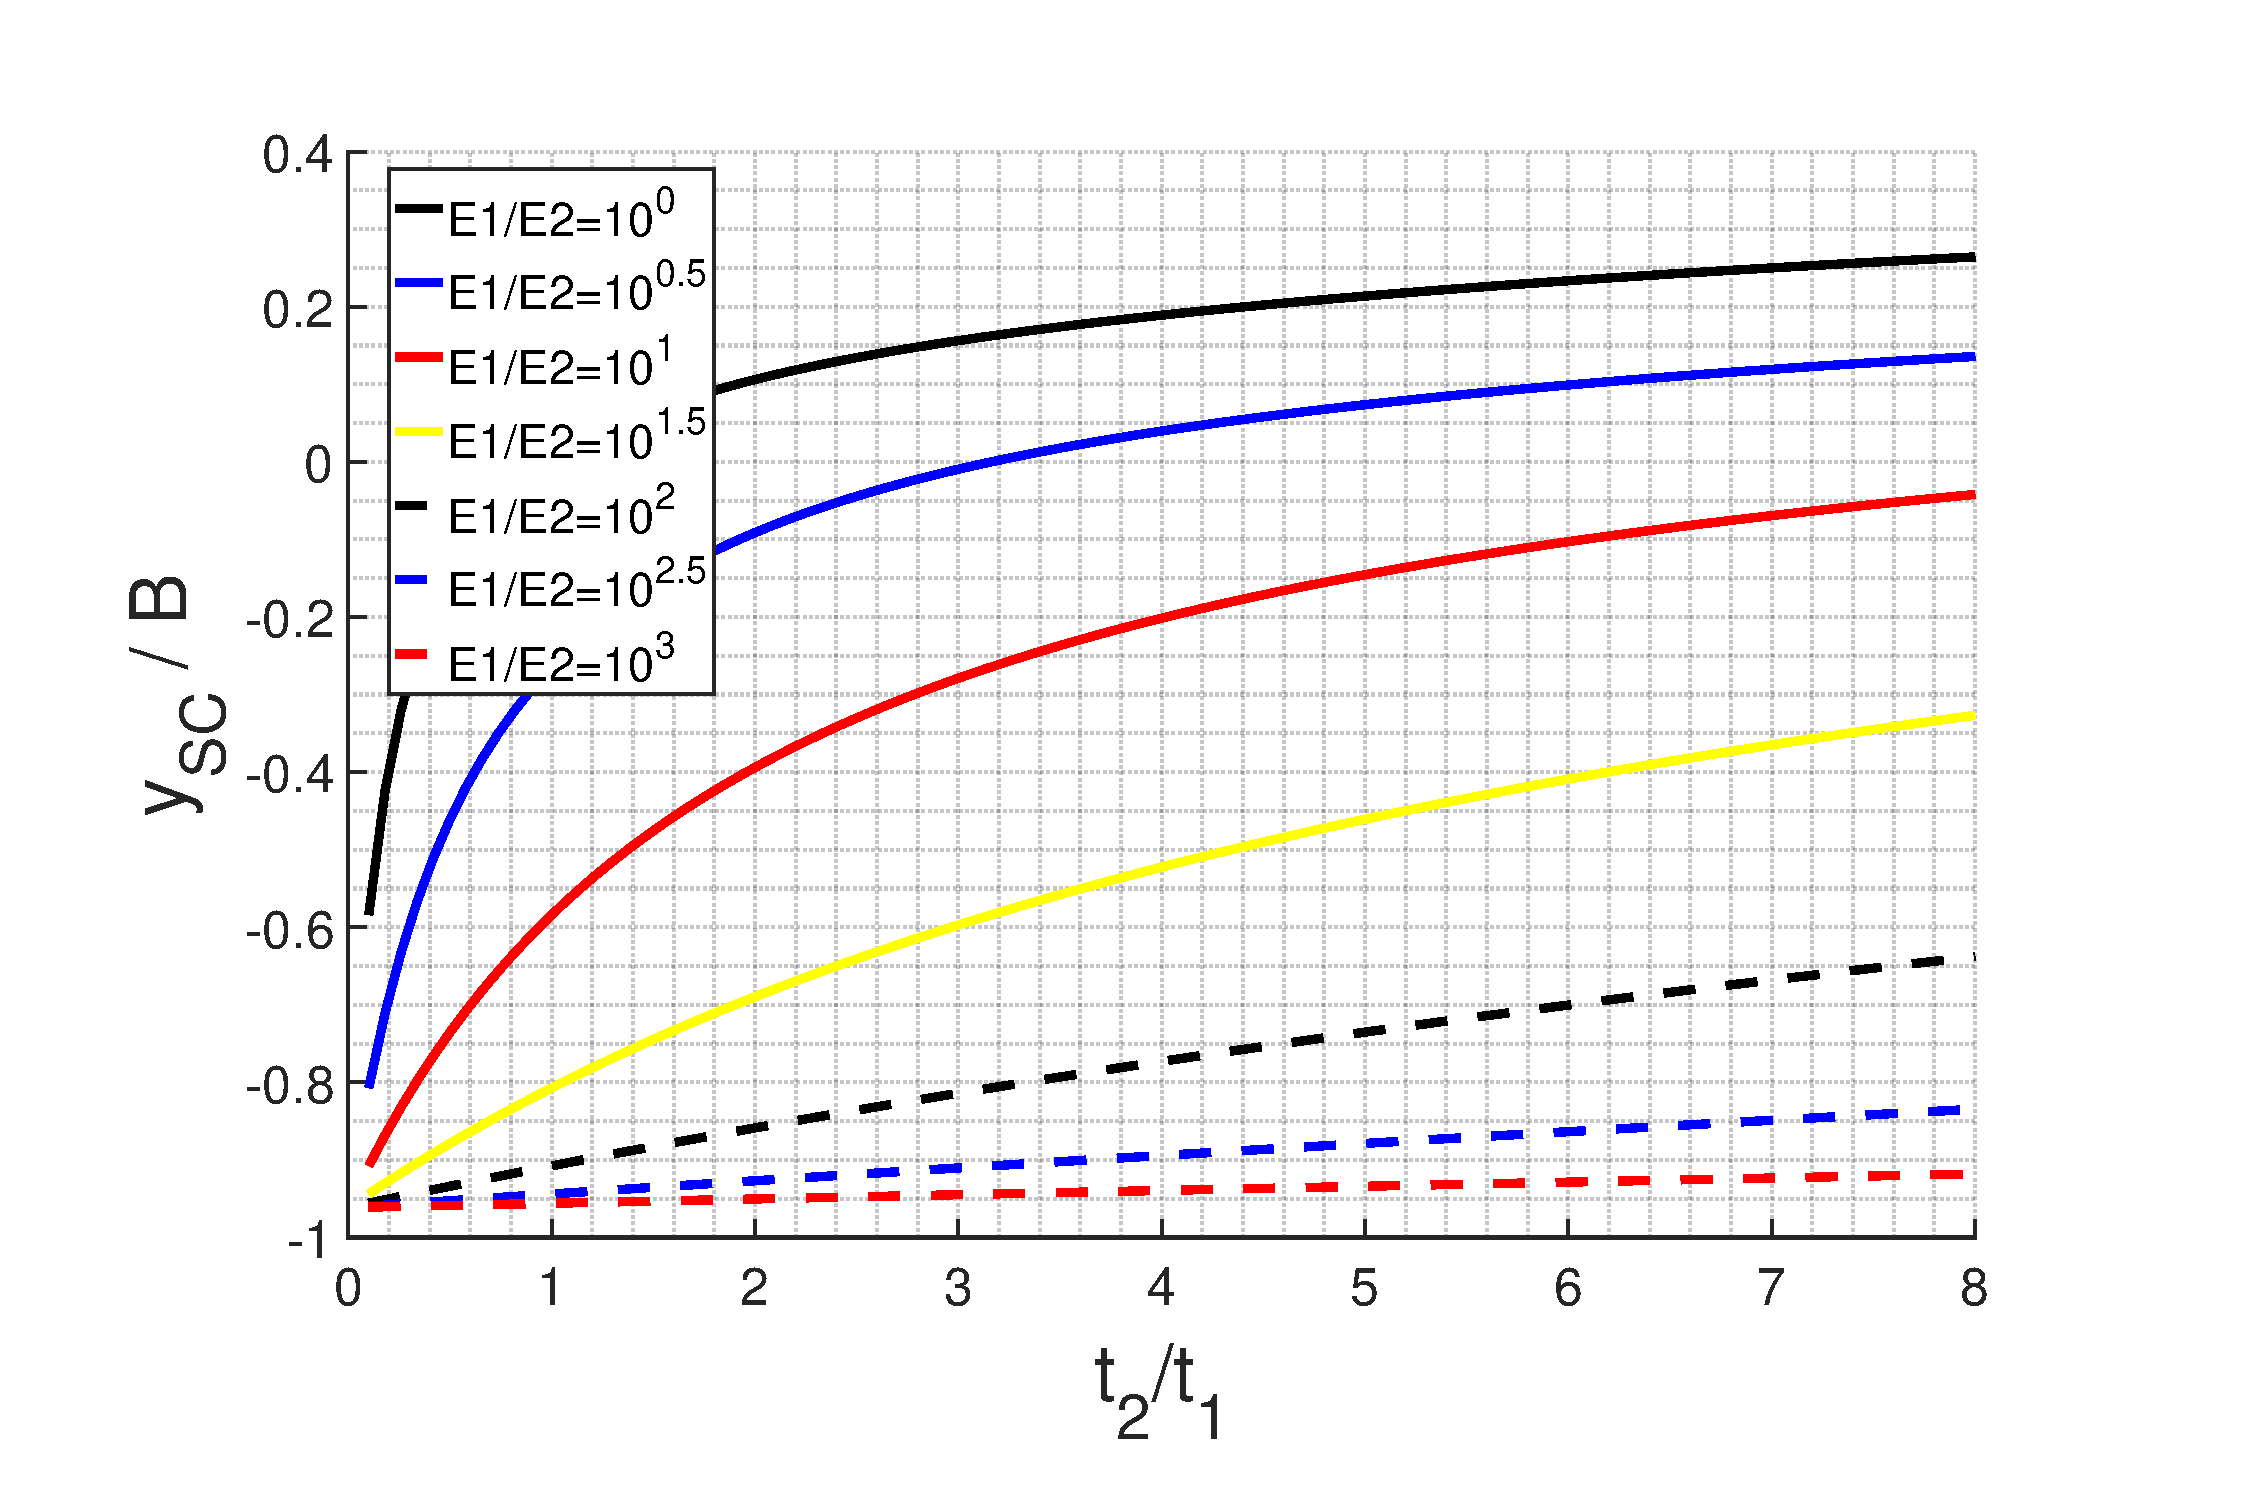
\includegraphics[width=0.8 \textwidth]{../../analytical/figures/SC-E1overE2-t2overt1}
  \caption[Influence of the wall thickness ratio $t_2/t_1$ on the dimensionless shear centre position $y_{SC}/B$]{Influence of the wall thickness ratio $t_2/t_1$ on the dimensionless shear centre position $y_{SC}/B$ shown for various values of the stiffness ratio $E_1/E_2$ ranging from $10^0$ to $10^3$. }\label{fig:SC-E1overE2-t2overt1}
\end{figure}

\begin{figure}[!htpb] %E I_y = \Phi_y versus B/H
  \centering
  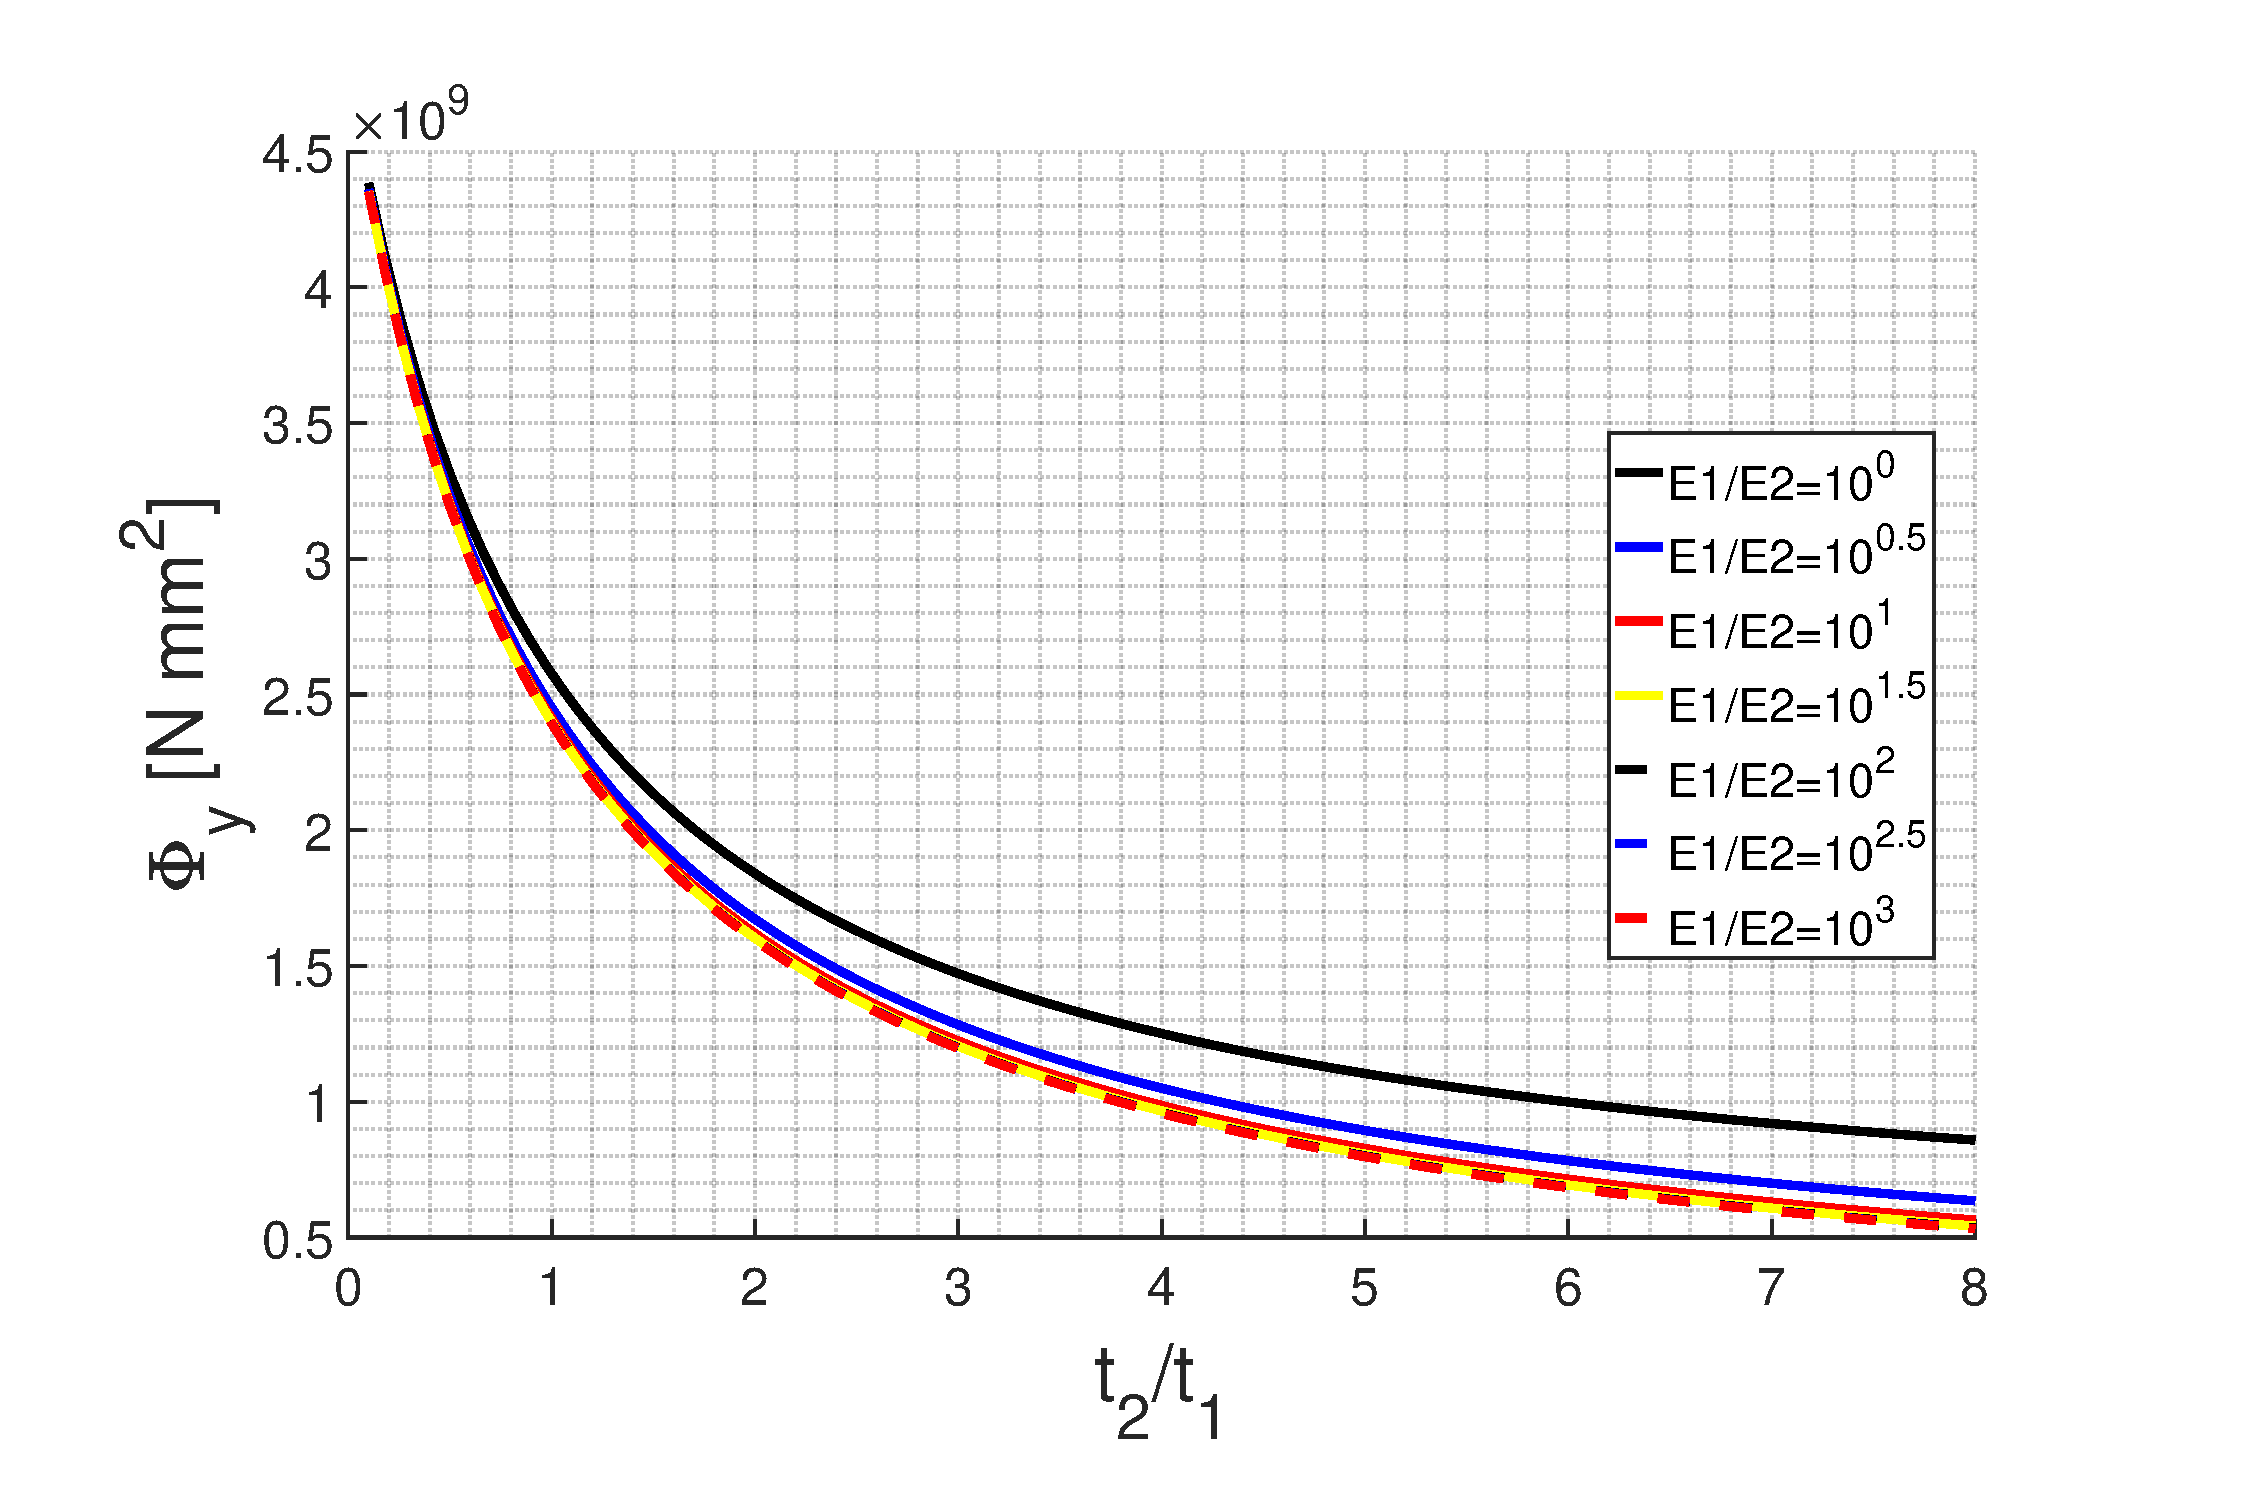
\includegraphics[width=0.8 \textwidth]{../../analytical/figures/EIy-E1overE2-t2overt1}
  \caption[Influence of the wall thickness ratio $t_2/t_1$ on the flexural stiffness $EI_y$]{Influence of the wall thickness ratio $t_2/t_1$ on the flexural stiffness $EI_y = \Phi_y$ shown for various values of the stiffness ratio $E_1/E_2$ ranging from $10^0$ to $10^3$. }\label{fig:EIy-E1overE2-t2overt1}
\end{figure}

\subsubsection{Discussion of the results} \label{subsubsec:results_parametricStudy}

The maximum torsional stiffness $G I_t$ as a function on the cross-sectional aspect ratio $B/H$ can be visualized in Figure \ref{fig:GIt-E1overE2-BoverH}. It can be seen that it appears for $B/H = 1$ when $E_1/E_2 = 1$. Therefore, as it is also shown in \cite{Raither_basic}, the closer the torsional stiffness to the doubly symmetric case, the higher its torsional stiffness. However, when $E_1/E_2 > 10$, the maximum torsional stiffness is shown to appear for $B/H > 1$.

In Figure \ref{fig:SC-E1overE2-BoverH} it can be seen that for values $E_2 \ll E_1$, the shear centre position $y_{SC}$ is approximately constant for $B/H$ variations. However, as the value of $E_1/E_2$ decreases, the influence of the ratio $B/H$ increases. The first behavior shows that the beam becomes  

%Comparison of the torsional compliance at the tip against stiffness ratio

\section{Computational model} \label{sec:computationalModel}

% Description of the model
%   Include all the parts of the model: C-box shape, inner box, chiral lattice
%   Figure of the model
% Parameters included
% 